\documentclass[conference,compsoc]{IEEEtran}
\newcommand\tab[1][0.75cm]{\hspace*{#1}}
\usepackage[utf8]{inputenc}
\usepackage[table,xcdraw]{xcolor}

%\ifCLASSOPTIONcompsoc
   \usepackage[nocompress]{cite}
%\else
 
\usepackage{cite}
\usepackage{url}
%\fi


\usepackage[pdftex]{hyperref}


% *** GRAPHICS RELATED PACKAGES ***

\ifCLASSINFOpdf
   \usepackage{graphicx}
   \graphicspath{{files/}}
  
\else
 
\fi
% correct bad hyphenation here
\hyphenation{op-tical net-works semi-conduc-tor}

%********** Começo do documento ************88

\begin{document}



\title{\resizebox{!}{0.75cm}{Ponto de controle 3}\\Reconhecimento facial em tempo real aplicado no Restaurante Universitário da Faculdade Gama.}



\author{
\IEEEauthorblockN{João Vitor Rodrigues Baptista}
\IEEEauthorblockA{15/0013329\\UnB - FGA \\
Brasília, Brasil \\
Email: jvrbaptista@live.com }
\and
\IEEEauthorblockN{Igor Sousa Nunes de Oliveira}
\IEEEauthorblockA{15/0011971\\
UnB - FGA \\
Brasília, Brasil\\
Email: igorsno97@gmail.com }}
\maketitle

% As a general rule, do not put math, special symbols or citations
% in the abstract

\begin{abstract}
Aplicação de monitoramento facial em tempo real no Restaurante Universitário da Faculdade Gama utilizando Raspberry pi para melhorar a eficiência do sistema e evitando problemas no acesso de usuários. \cite{referencia:3} 
\end{abstract}
\IEEEpeerreviewmaketitle
\section{Introdução}
Sistemas de controles de acesso são uma ferramenta muito importante na contemporaneidade para a segurança de ambientes controlados, produtos, pessoas ou para de maneira simples um controle de tempo dos usuários do sistema. \cite{referencia:7}

Com o passar do tempo notou-se que uma boa forma de identificação seria através de padrões do ser humano de maneira que a chave de acesso sempre estaria com usuário. Um dos padrões bastante associados com a identificação foi a digital, e desde cedo estudada para se entender padrões já que a  mesma é diferente para cada pessoa, sensores biométricos se tornaram bastante utilizados desde celulares até mesmo cofres. Um padrão que está sobre um grande estudo na contemporaneidade são padrões reconhecidos por imagem como a face e em certas aplicações até mesmo a leitura de padrões na iris do usuários.\cite{referencia:7}

A tecnologia entrou em um padrão de evolução buscando maior conforto, acessibilidade, velocidade e segurança
para seus usuários, o reconhecimento facial se tornou uma poderosa ferramenta na aquisição de dados por 
não precisar de módulos sensores de uso específicos como o leitor biométrico. 

Em países como a China onde o investimento na área de segurança e processamento digital de imagens conseguiram criar uma rede de câmeras que identificam pessoas a distancia, então o processo de transformar o usuário na própria chave do sistema
foi a melhor saída para uma maior segurança do sistema, praticidade e até mesmo melhoras no fluxo de filas em 
ambientes controlados entre outros.\cite{referencia:4} \cite{referencia:5} 

\section{Justificativa}
Na  contemporaneidade o grande fluxo de pessoas em diversos ambientes controlados levantou questões sobre a eficiência dos métodos utilizados, em geral existe um custo associado individualmente para cada usuário possua uma chave(no caso de cartões, tarjas magnéticas, transponders entres outros).  A segurança é uma outra característica fundamental ao ambiente de maneira que os métodos comumente utilizados possuem uma maior probabilidade de serem fraudados.

Motivado pela modernização implementada no controle de acessos a escolha de uma parâmetro de identificação biométrico se torna de grande utilidade como chave do sistema, pois o usuário se torna chave do sistema o que tira do projeto um custo adicional pertencente a cada passe que deve utilizado individualmente para um controle mais efetivo do ambiente.

Com uma pesquisa sobre o custo beneficio de cada tipo de leitura biométrica a escolhida como tema deste projeto pelo baixo custo e boa eficiência de maneira que uma das suas principais vantagens é a facilidade de identificação de fraude por terceiros que estejam no mesmo lugar. Diante do exposto a utilização do reconhecimento facial torna mais cômodo para os usuários e para o proprietário do sistema, devido uma maior eficiência e automatização do mesmo em comparação a outros métodos.
 
 \section{Objetivos}
Tornar o controle de acesso ao Restaurante Universitário da Faculdade Gama eficientes tornando o fluxo de pessoas que entram mais rápido e automatizando o controle de usuários.
Identificar as pessoas que entram e saem além de poder ter
controle dos tempos de acessos de cada pessoa individualmente e armazenar em um banco de dados.
Monitorar pessoas que tentem entrar no ambiente de forma
indevida e impedir a entrada de usuários quem não tenham a
devida autorização.

\begin{figure}[!ht]
		\centering
		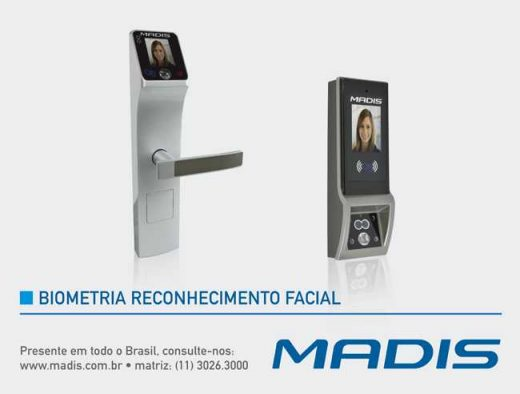
\includegraphics[scale=0.25]{exemplo.jpg}
		\caption{Produto semelhante já encontrado no mercado \cite{referencia:8}}
		%\label{Rotulo}
\end{figure}

 \section{Tabela de materiais utilizados}
\begin{table}[!ht]
\begin{tabular}{|c|c|c|c|}
\hline
{\color[HTML]{000000} \textbf{UND}} & {\color[HTML]{000000} \textbf{Materiais}}                                                            & {\color[HTML]{000000} \textbf{Fabricante}} & {\color[HTML]{000000} \textbf{Preço}} \\ \hline
{\color[HTML]{000000} 1}            & {\color[HTML]{000000} Raspberry pi 3b}                                                               & {\color[HTML]{000000} Raspberry}           & {\color[HTML]{000000} R\$ 200,00}     \\ \hline
{\color[HTML]{000000} 1}            & {\color[HTML]{000000} Cabo HDMI}                                                                     & {\color[HTML]{000000} -}                   & {\color[HTML]{000000} R\$15,00}       \\ \hline
{\color[HTML]{000000} 1}            & {\color[HTML]{000000} Monitor/Display}                                                               & {\color[HTML]{000000} -}                   & {\color[HTML]{000000} -}              \\ \hline
{\color[HTML]{000000} 1}            & {\color[HTML]{000000} Cartão microSD}                                                                & {\color[HTML]{000000} SanDisk}             & {\color[HTML]{000000} R\$100,00}      \\ \hline
{\color[HTML]{000000} 1}            & {\color[HTML]{000000} \begin{tabular}[c]{@{}c@{}}Mini trava elétrica \\ Solenóide 12 V\end{tabular}} & {\color[HTML]{000000} -}                   & {\color[HTML]{000000} R\$ 35,00}      \\ \hline
{\color[HTML]{000000} -}            & {\color[HTML]{000000} Jumpers}                                                                       & {\color[HTML]{000000} -}                   & {\color[HTML]{000000} R\$ 5,00}       \\ \hline
{\color[HTML]{000000} 1}            & {\color[HTML]{000000} \begin{tabular}[c]{@{}c@{}}Módulo Câmera \\ Raspberry 3\end{tabular}}          & {\color[HTML]{000000} Raspberry}           & {\color[HTML]{000000} R\$ 45,00}      \\ \hline
{\color[HTML]{000000} 1}            & {\color[HTML]{000000} Módulo Relé 5V}                                                                & {\color[HTML]{000000} -}                   & {\color[HTML]{000000} R\$ 5,00}       \\ \hline
{\color[HTML]{000000} 1}            & {\color[HTML]{000000} Fonte 12 V}                                                                    & {\color[HTML]{000000} -}                   & {\color[HTML]{000000} R\$ 10,00}      \\ \hline
\end{tabular}
\end{table}

 \section{Relação de custo}
 Até o presente momento foi-se gasto em torno de R\$ 400,00 para a construção e desenvolvimento do projeto, o custo pode ser reduzido com compras de componentes em maiores quantidades ou mesmo com importações de peças como a própria raspberry, o estudo sobre uma melhor compra dos materiais utilizados torna o hardware do sistema mais barato fazendo de maneira simples que o produto final tenha um custo mais competitivo e com isso uma análise de mercado possa ser feita comparando o produto desenvolvido com outros concorrentes utilizados em maior escala para o controle e segurança dos ambientes.
 
Um ponto que se encontra em estudo e precificação no momento do projeto é a precificação do produto final para se entender o melhor dimensionamento de monitor para ter um balanço sobre o custo do mesmo e até consumo de energia, para que o produto seja viável com um maior custo beneficio. O uso de um pequeno protótipo se fez necessário para que a ideia do sistema seja de fato melhor mostrada até mesmo para possíveis clientes, o custo do mesmo não foi associada ao projeto, pois é apenas e um representativo de um sistema onde poderia ser aplicado, com uma real demanda do produto a analise de possíveis designs entre outros se torna necessária.

 \section{Hardware}
 
 Foi passado e configurado todos os APIs utilizados para o processamento de imagens para o microcontrolador raspberry pi 3 B. Recopilou-se todos os códigos e banco de dados para a arquitetura do processador. 
 
 \begin{figure}[!ht]
		\centering
		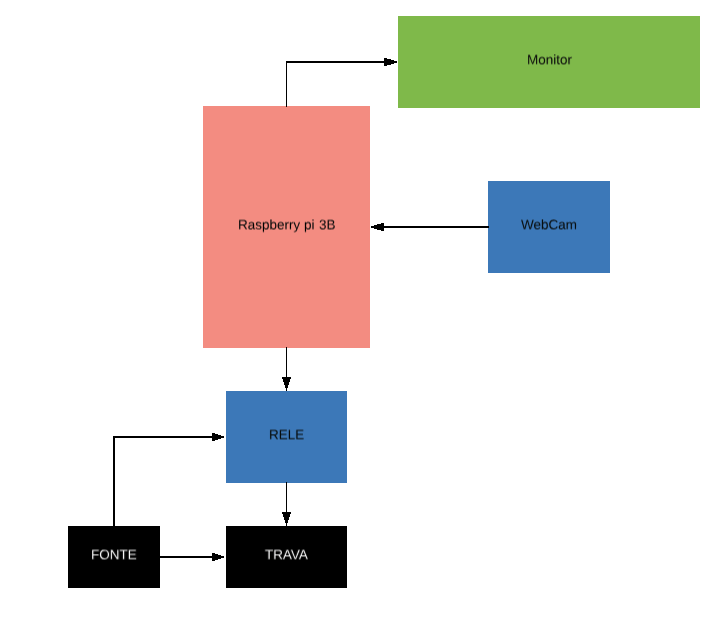
\includegraphics[scale=0.25]{diagrama_de_hardware.png}
		\caption{Diagrama de Hardware}
		%\label{Rotulo}
\end{figure}

Como esta indicado no diagrama de hardware do projeto. Ligou-se a raspberry pi 3B como entrada em um monitor qualquer para melhorar a interação entre o usuário e o sistema, já que será indicado se o usuário foi reconhecido. A webcam foi ligada como entrada do sistema, pois a partir dos dados de entrada providos o sistema faz o julgamento se o usuário esta ou não cadastrado no banco.
	
	Uma vez que o usuario foi reconhecido e tem creditos o suficiente o sistema manda um sinal para abrir um rele 5V que esta sendo a chave de uma tranca solenoide de 12v. 




 \section{Software}

O software tem como o principio básico três partes que consiste em cadastrar o aluno, reconhecer a imagem gravada com as imagens do banco de dados e alteração do banco de dados.

\begin{figure}[!ht]
		\centering
		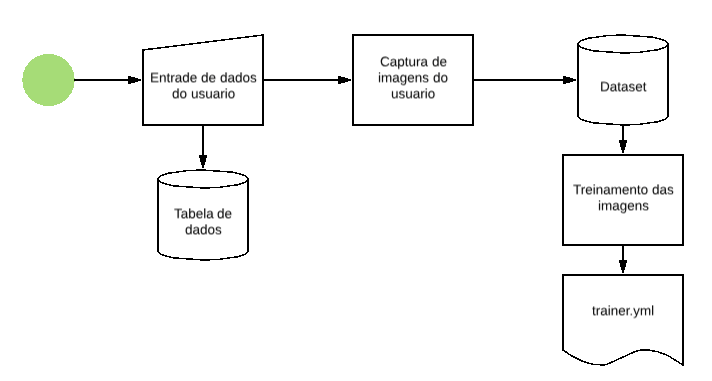
\includegraphics[scale=0.25]{Cadastro.png}
		\caption{Fluxograma do funcionamento do cadastro.}
		%\label{Rotulo}
\end{figure}

Na figura 1 é apresentado o fluxo de cadastro, onde o aluno digita o nome e a matricula, em seguida são tiradas 30 fotos que são salvas em um dataset com a posição do vetor posição como nome, em seguida são feitas os processamentos de imagens da biblioteca opencv.

\begin{figure}[!ht]
		\centering
		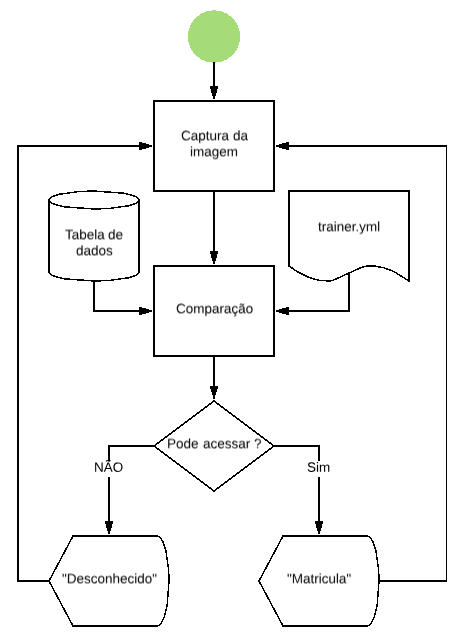
\includegraphics[scale=0.25]{Reconehcimento.png}
		\caption{Fluxograma do funcionamento do reconhecimento da biblioteca opencv.}
		%\label{Rotulo}
\end{figure}

Na figura 2 é mostrado o fluxo de reconhecimento de imagem. A partir do arquivo gerado pelo treinamento do dataset, a biblioteca opencv faz o reconhecimento entre o que esta sendo gravado e as imagens que foram treinadas com uma precisão ajustável, que depende tanto da qualidade da câmera, como das condições do ambiente. 

\begin{figure}[!ht]
		\centering
		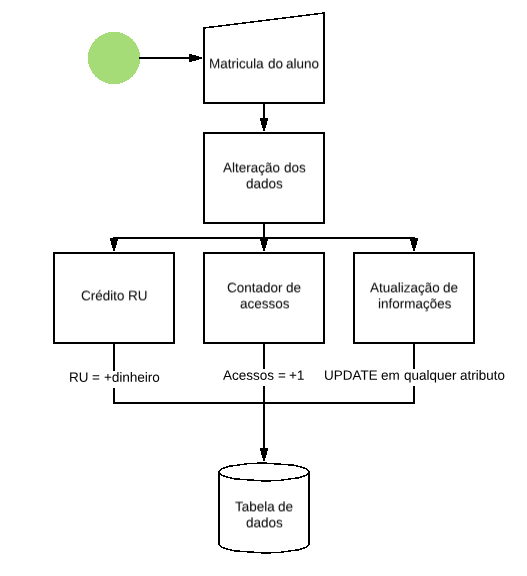
\includegraphics[scale=0.25]{Banco_de_dados.png}
		\caption{Fluxograma do funcionamento banco de dados.}
		%\label{Rotulo}
\end{figure}

A figura 3 mostra algumas funções de manipulação do banco de dados que serão usadas futuramente para o controle do sistema de acesso. As funções implementadas são: Adicionar crédito, contador de acessos e apagar um cadastro. Será necessário implementar mais funcionalidades.

O banco de dados esta organizado de acordo com a tabela de CADASTROS que possui cinco atributos, ID, NOME, MATRICULA, RU e ACESSOS como mostrado na figura 4. Podendo, se necessário, ser adicionado novos atributos.  


 \begin{figure}[!ht]
		\centering
		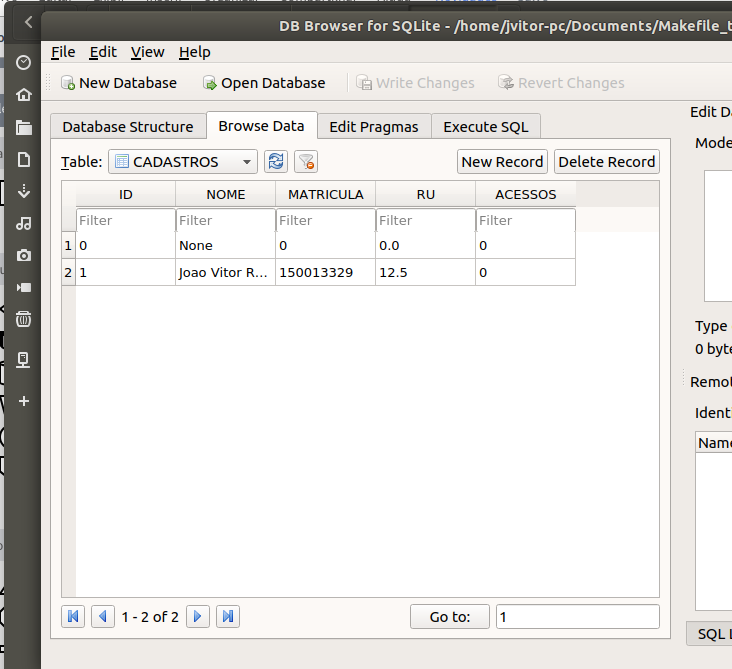
\includegraphics[scale=0.25]{infra_database.png}
		\caption{Atributos do banco de dados.}
		%\label{Rotulo}
\end{figure}

Todos os codigos e figuras estão no repositório no GitHub, através do link:
\href{https://github.com/helpthx/Sistemas_Embarcados/tree/master/2_PCs/Ponto_de_Controle_2/Arquivos_SQL}{helpthx}

\section{Requisitos}
\begin{itemize}
   \item Um microcontrolador no qual a escolha de projeto é o Raspberry pi 3 B. 
   \item Um módulo de câmera para a Raspberry.
   \item Um display para se mostrar as informações necessárias.
   \item Uma estrutura para proteger o sistema.
   \item Cabo HDMI.
   \item Modulo rele 5V.
   \item Fonte de alimentação.
   \item Tranca solenoide 12V
   \item Conexão com a internet.
   \item Software de reconhecimento facial.
   \item Software  para criação de logs e registros.
   \item  Infraestrutura do servidor para criação e alteração do banco de dados.
   \item Banco de dados para guardar informações do usuário(Fotos, créditos e acessos).
   \item Testador de continuidade.
 \end{itemize}
 
\section{Benefícios}
Processo com maior segurança para os usuários, onde não é necessário  memorizar senhas ou carregar algum tipo de chave, o traço pessoal é mais difícil de ser clonado ou copiado o que trás maior segurança para todos os usuários do sistema.

Custo semelhante ou inferior ao de sistemas de controles de acessos, valorização da modernização, melhoria do design e apresentação do ambiente.

\section{Resultados}

Foi verificado uma queda de processamento em comparação com o sistema em um notebook, porem é totalmente possível utilizar a raspberry para essa aplicação. Nos testes iniciais foi utilizado uma webcam com uma qualidade inferior a qualidade da câmera própria da raspberry e foram tiradas apenas 30 fotos de base, contudo os resultados foram satisfatórios pois foi alcançado um nível de 70\% de confiabilidade entre o que foi cadastrado e a entrada da webcam.

\begin{figure}[!ht]
		\centering
		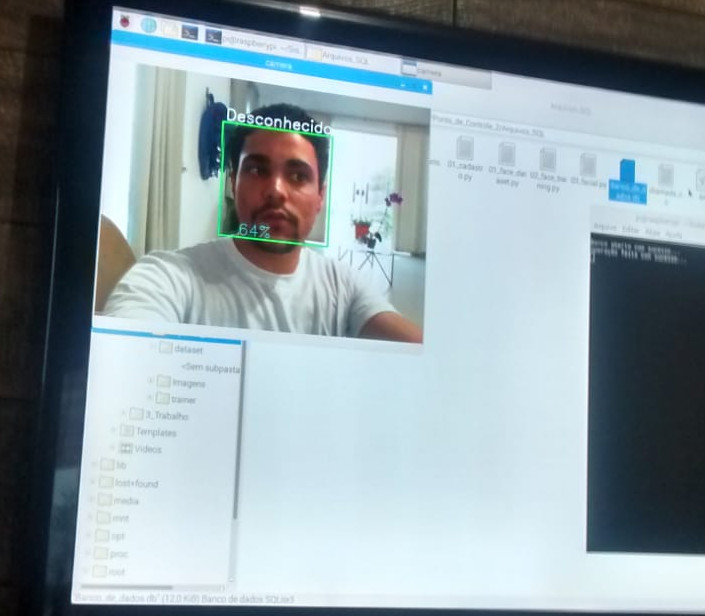
\includegraphics[scale=0.20]{teste1_1.jpeg}
		\caption{Confiabilidade menor do que 70\% sistema exibe "Desconhecido"}
		%\label{Rotulo}
\end{figure}

	Visto que será implementada a câmera própria da raspberry e serão feitos  testes sobre proporção de fotos e a confiabilidade do sistema. Possivelmente, o sistema poderá ter 75\% de confiabilidade até o protótipo final.
	
	\begin{figure}[!ht]
		\centering
		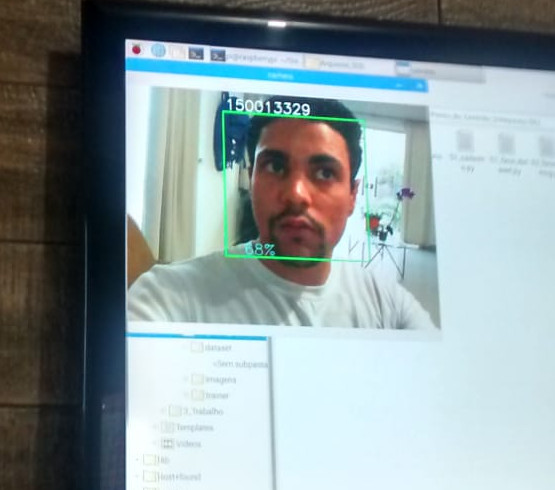
\includegraphics[scale=0.25]{teste2_1.jpeg}
		\caption{Confiabilidade maior do que 70\% sistema exibe "Matricula"}
		%\label{Rotulo}
\end{figure}
	
	O sistema de banco de dados esta totalmente funcional e operando dentro do esperado. Atualmente, existem 5 funcionalidades: Criar um banco novo, Adicionar créditos do RU, Remover Usuário Cadastrado, Adicionar Usuário e contador de acessos. Essas funções serão implementadas no sistema de gerenciamento que será acessado através de uma aplicação web.  
%---------------------  ----------------------

%\section{Materiais Utilizados}
%TABELAS AQUI

%\begin{table}[tbp]
%\caption{Tabela 1 - Exemplo}
%\label{my-label}
%\begin{tabular}{ccccc}
%\textbf{Nome}   & \textbf{Nome1} & \textbf{Nome2} & \textbf{Nome3} & \textbf{Nome4} \\
%\textbf{Nome11} & 1              & 2              & 3              & 4              \\
%\textbf{Nome21} & 5              & 6              & 7              & 8              \\
%\textbf{Nome31} & 9              & 10             & 11             & 12            
%\end{tabular}
%\end{table}
%---------------------  ----------------------

%\section{Hardware e Software}

%---------------------  ----------------------
%\subsection{Descrição do Hardware}

%Como é observado no diagrama de blocos, é necessária uma fonte externa para acionar a trava solenoide, pois os 3 volts fornecidos pela placa não é suficiente para fazer o acionamento da trava.

%\begin{figure}[!ht]
%		\centering
%		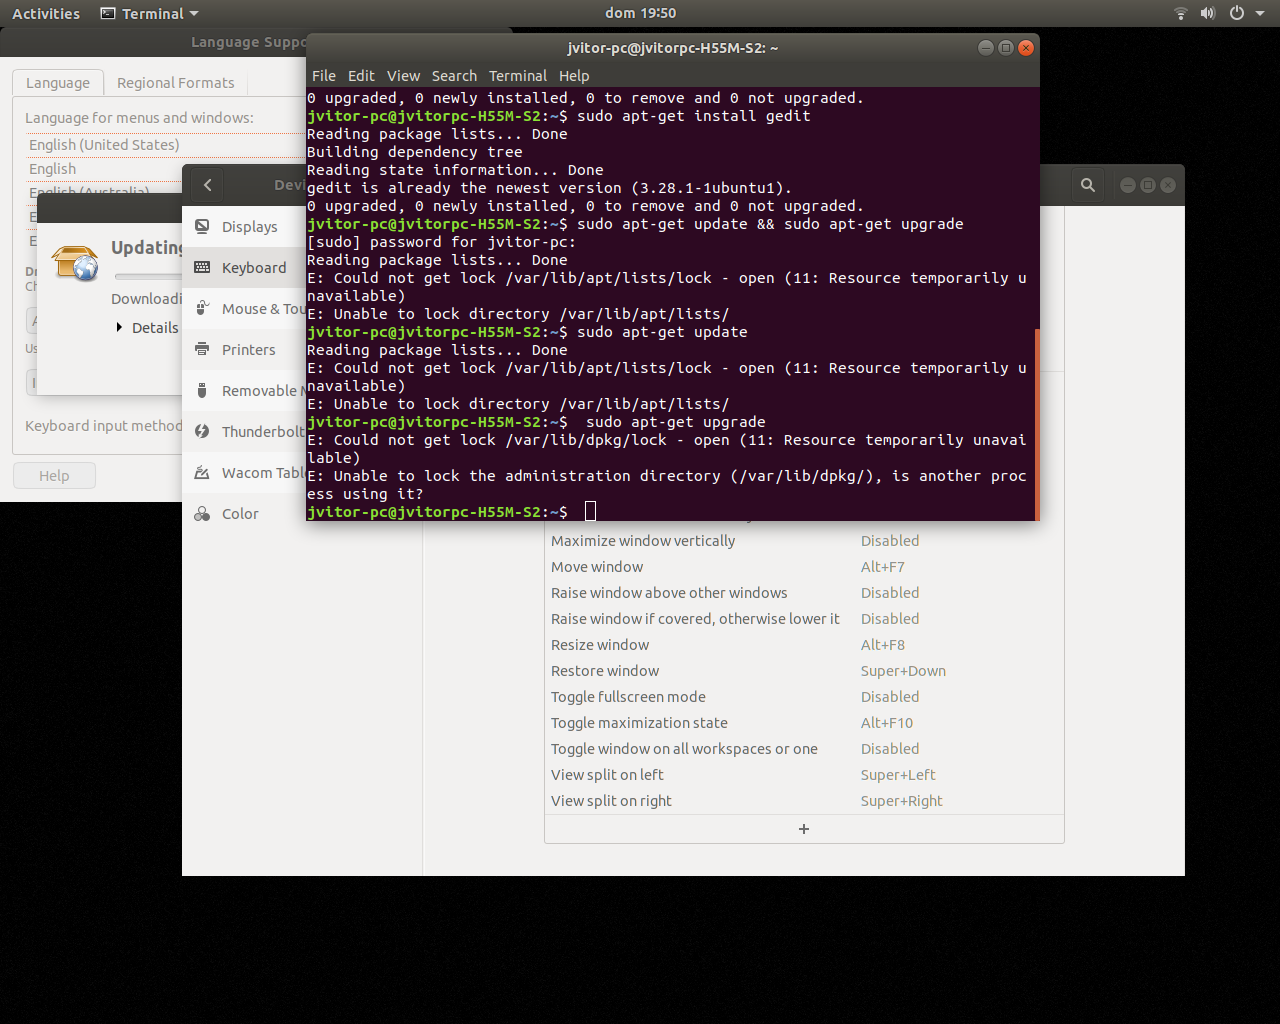
\includegraphics[scale=0.15]{nome_da_figura.png}
%		\caption{Figura 1.}
		%\label{Rotulo}
%\end{figure}

%O resultado foi o esperado, ao passar o tag no leitor RFID, gerou-se um sinal para o relê abrir a tranca eletrônica, através da alimentação de uma bateria de 9 – 12V. 
%Display de Cristal Liquido: Pode ser facilmente implementado no MSP430 utilizando a biblioteca "LiquidCrystal.h". O display será utilizado para exibir as mensagens:

%---------------------  ----------------------


%\subsection{Descrição do Software}
%Para melhor ilustrar o caminho logico deste sistema, foi construído um Diagrama Logico na imagem 5. Para mostrar de maneiras simples a ideia lógica do sistema proposto.
% \begin{figure}[!ht]
%		\centering
%		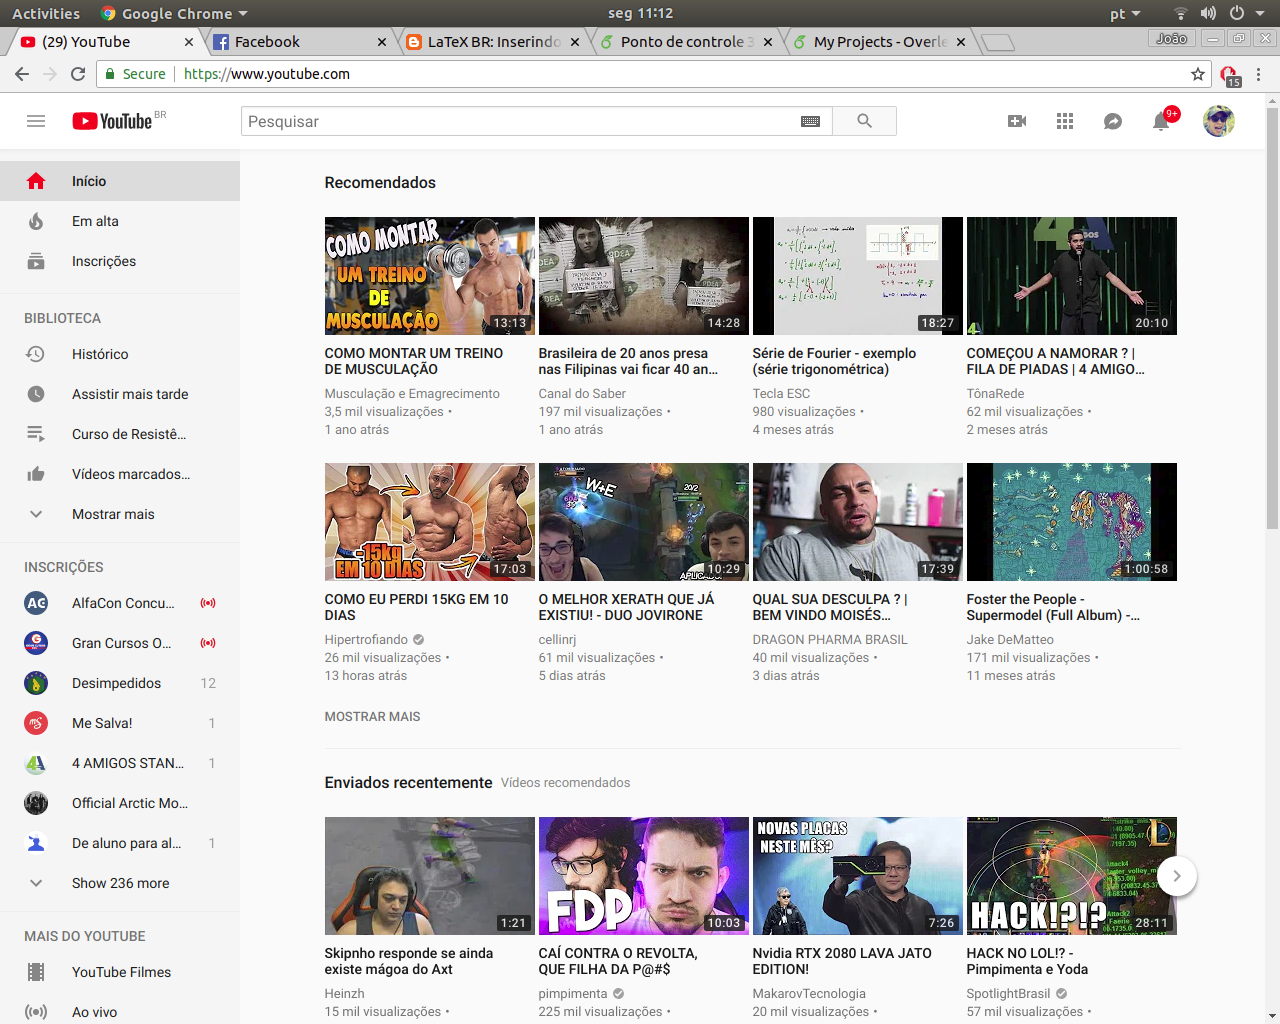
\includegraphics[scale=0.15]{nome_da_figura1.png}
%		\caption{Figura 1}
		%\label{Rotulo}
%\end{figure}

%O Sistema consiste nos seguintes passos:

%\tab 1. Iniciar a comunicação UART com o RC522. Exibindo “RFID LOADING...” ao iniciar.

%\tab 2. Quando o sistema estiver pronto e iniciado exibir “PASSE O CARTÃO”.

%\tab 3. Ler o conteúdo do cartão ou tag.

%\tab 4. Julgar se o cartão ou tag, pode ou não destravar o sistema.

%\tab 5. Destrava o sistema e envia um sinal para o rele, exibe  “BEM VINDO USUARIO”, espera 7 segundos e vai para o loop de leitura.

%\tab 6. Trava o sistema quando o cartão não tem acesso, exibe “ACESSO NEGADO”, volta para o loop de leitura. 



%\begin{figure}[!ht]
%		\centering
%		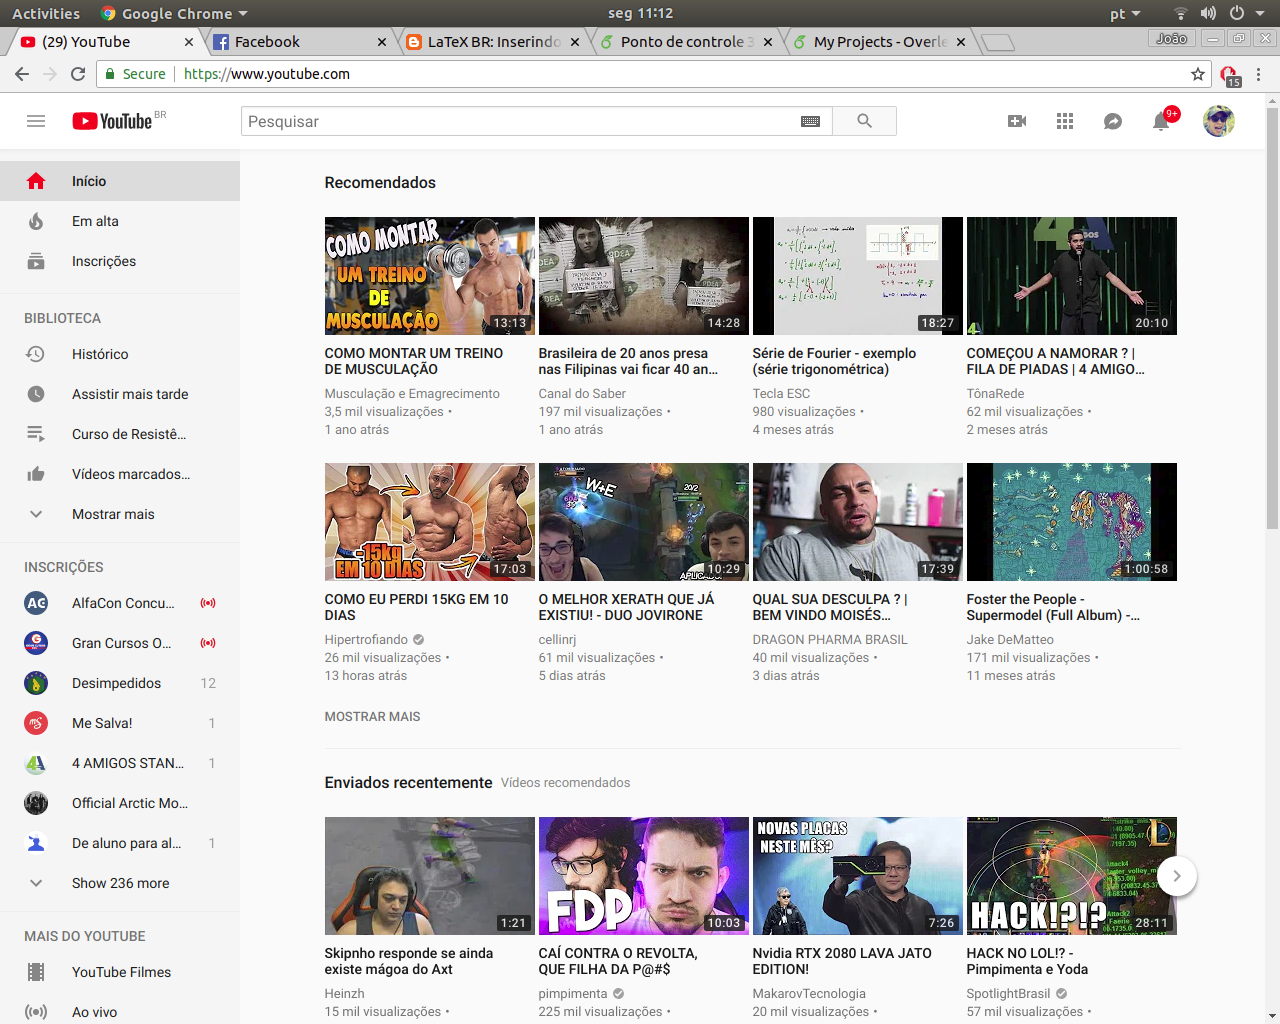
\includegraphics[scale=0.15]{nome_da_figura1.png}
%		\caption{Figura 1}
		%\label{Rotulo}
%\end{figure}

%Os códigos e as figuras estão no GitHub, através do link:\href{https://github.com/helpthx}{https://github.com/helpthx}

%---------------------  ----------------------

%\section{Resultado}
%Os resultados foram conforme o esperado ao se juntar todos os componentes, entretanto houve algum problema na comunicação com o display 16x2, o qual não exibe as mensagens de trava e destrava do sistema de maneira correta, ou seja, em certos momentos caracteres estranhos são mostrados no display. Porem a comunicação entre o RC522, MSP430 e o rele esta totalmente funcional e a trava esta se comportando como deveria. Para os próximos passos será corrigido o problema do display e possivelmente adicionado mais funções ao sistema.

%\begin{figure}[!ht]
%		\centering
%		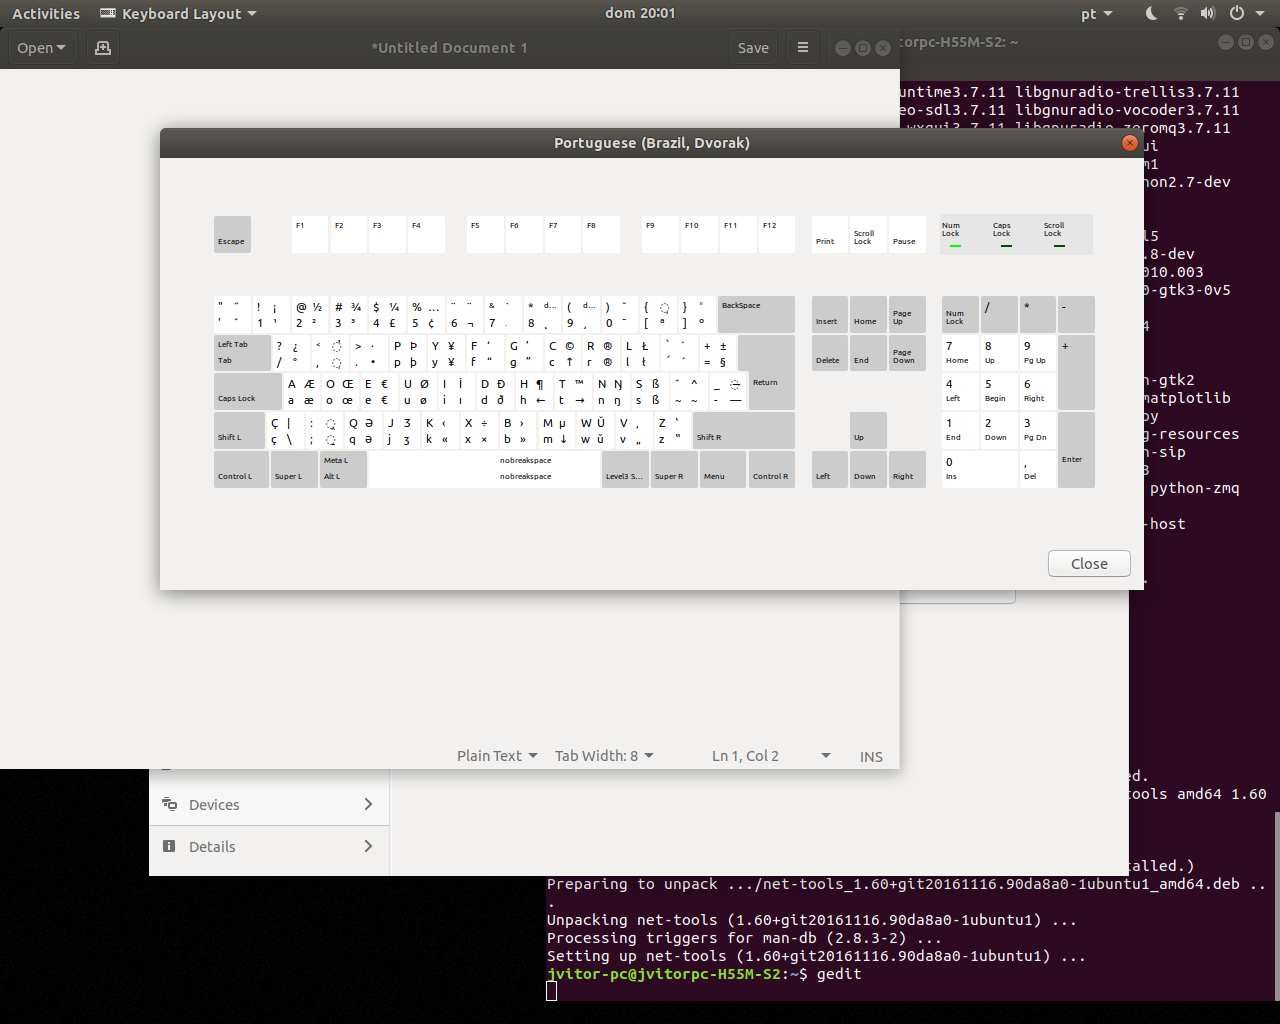
\includegraphics[scale=0.15]{nome_da_figura3.png}
%		\caption{Figura 3}
		%\label{Rotulo}
%\end{figure}

%---------------------  ----------------------

%\section{Relação de Custo}
%Até o presente momento se foi gasto em torno de R\$214,10 para o projeto, o que pode ser extremamente reduzido se as peças fossem compradas com certa antecipação, o MSP comprado direto pelo fornecedor a Texas, dessa maneira fazer com que o preço do projeto reduzido em mais de 50\% do valor atual, os outros componentes se comprando em grandes quantidades consegue-se uma grande redução de preços, o que viabilizaria a construção em maior escala do projeto com um menor preço e com certas melhorias uma possível entrada na concorrência de vendas de produtos pensados para segurança e controle de ambientes, como sendo uma alternativa de baixo custo que poderia ser modificada com necessidades do próprio cliente. \cite{referencia:1}



%-------------------- REFERÊNCIA -----------------

\begin{thebibliography}{1}


%\bibitem{IEEEhowto:kopka}
%H.~Kopka and P.~W. Daly, \emph{A Guide to \LaTeX}, 3rd~ed.\hskip 1em plus
 % 0.5em minus 0.4em\relax Harlow, England: Addison-
%FALTA ARRUMAR AS REFERÊNCIAS


\bibitem{referencia:2}
{TIWARI, Shantnu
\emph{Face Detection in Python Using a Webcam.},
 {Disponivel em:\url{<https://realpython.com/face-detection-in-python-using-a-webcam/>}},{Acesso em: 01 set. 2018.}
}

\bibitem{referencia:3}
{MJROBOT, MJRoBot.
\emph{Real-Time Face Recognition: An End-to-End Project.},
 {Disponivel em:\url{<https://www.hackster.io/mjrobot/real-time-face-recognition-an-end-to-end-project-a10826>.}},{Acesso em: 01 set. 2018.}
}

\bibitem{referencia:4}
{VICENTIN, TISSIANE.
\emph{Projeto usa Raspberry e reconhecimento facial para medir produtividade.},
 {Disponivel em:\url{<https://www.tecmundo.com.br/software/126916-projeto-usa-raspberry-reconhecimento-facial-medir-produtividade.htm>}},{Acesso em: 01 set. 2018.}
}

\bibitem{referencia:5}
{CASSITA, DANIELLE.
\emph{Reconhecimento facial ajuda polícia a identificar suspeito em festival. 2018.},
 {Disponivel em:\url{<https://www.tecmundo.com.br/software/133803-reconhecimento-facial-ajuda-policia-identificar-suspeito-festival.htm>.}},{Acesso em: 01 set. 2018.}
}

\bibitem{referencia:6}
{CHOWDHURY, Nasimuzzaman.
\emph{Access Control of Door and Home Security by Raspberry Pi Through Internet. 2018.},
 {Disponivel em:\url{<https://www.ijser.org/researchpaper/access-control-of-door-and-home-security-by-raspberry-pi-through-internet.pdf>.}},{Acesso em: 01 set. 2018.}
}

\bibitem{referencia:7}
{AXIS, Communications.
\emph{Reconhecimento facial. },
 {Disponivel em:\url{<https://www.axis.com/pt-br/solutions-by-application/facial-recognition>}},{Acesso em: 01 set. 2018.}
}
\bibitem{referencia:8}
{INOVADOR DESDE 1923, MADIS.
\emph{Biometria Reconhecimento Facial.},
 {Disponivel em:\url{<https://www.madis.com.br/produtos/biometria-reconhecimento-facial/>.}},{Acesso em: 19 out. 2018.}
}


\end{thebibliography}




% that's all folks
\end{document}
